\section{XToolKit}
\markright{\arabic{section}. XToolKit}

XToolKitは、
ボタン、プルダウンメニュ、テキストwindowなどのGUI要素を使用して
GUI (Graphical User Interface)を作成するのを容易にするための
高レベルXwindowインターフェースである。
Xlibクラスとの大きな違いは、XToolKitがXserverから送られる
Xeventと一致するユーザーが定義した対話ルーチンを呼び出し、
それらの対話指向windowパーツと一致した外観を提供することである。
XToolKitに含まれるクラスは、以下の継承構造を持っている。
\begin{verbatim}
          xwindow
               panel
                    menubar-panel
                    menu-panel
                    filepanel
                    textviewpanel
                    confirmpanel
               panel-item
                    button-item
                         menu-button-item
                         bitmap-button-item
                         menu-item
                    text-item
                    slider-item
                    choice-item
                    joystick-item
               canvas
               textwindow
                    buffertextwindow
                         scrolltextwindow
                    textedit
               scroll-bar
                    horizontal-scroll-bar
\end{verbatim}

以下に示すxwindowクラスはXToolKitの5つの基本クラスである。
{\tt panel}, {\tt panel-item},
{\tt canvas}, {\tt textWindow}と{\tt scroll-bar}。
{\tt menubar-panel}と{\tt menu-panel}は、{\tt panel}の下に定義される。
新しいアプリケーションwindowを作り、イベントの上でそれを実行させるための
基本的な方策は、以下の通りである。
\begin{enumerate}
\item{\bf アプリケーションクラスの定義} アプリケーションクラスwindowは、
XToolKitの要素を置く能力を持つ{\bf panel}のサブクラスとして
定義されなければならない。
\item{\bf イベントハンドラの定義} アプリケーションクラスにおいて、
ボタンが押されたり、メニューアイテムが選択されたりしたときに
呼び出されるイベントハンドラを定義する。
イベントハンドラは、panel-itemの指定された引数を持つメソッドとして
定義すべきである。
\item{\bf サブパネルの定義} もし、{\tt menubar-panel}を使用するなら、
アプリケーションwindowの一番上におかれる。
したがって、{\tt :create-menubar}によって最初に作成されなければ
ならない。
同様に、{\tt menu-panel}は、その{\tt menu-panel}と関連する
{\tt menu-button-item}より前に定義する必要がある。
\item{\bf パネルアイテムの作成} {\tt button-item},
{\tt text-item}, {\tt slider-item}などのようなパネルアイテムは、
{\tt (send-super :create-item {\em class label object method})}によって
作成することができる。
上記で定義されたイベントハンドラは、それぞれのパネルアイテムと
接続される。
これらの初期化手続きは、アプリケーションwindowクラスの
{\tt :create}メソッドの中で定義すべきである。
必要なときはいつでもイベント送信を停止するための{\tt quit}ボタンを
定義することを忘れないこと。
どんな{\tt textWindow}と{\tt canvas}も、{\tt :locate-item}メソッドを経由して
アプリケーションwindowの中に置くことができる。
\item{\bf window全体の作成} {\tt :create}メッセージをアプリケーション
クラスに送ることで、windowにXToolKitの要素を正しく置いたアプリケーション
windowを作成する。
%If you do not like the default placement, add {\tt :x} and {\tt :y}
%parameters at the creation of each component.
\item{\bf イベント送信の実行} Xserverからイベントを受け、一致する
windowに配るためには、{\tt window-main-loop}を実行すること。
Solaris2上では、イベントを配るための異なったスレッドである
{\tt window-main-thread}で実行する。
{\tt window-main-thread}では、最上位レベルの対話が活きている。
{\tt window-main-thread}を2回以上実行してはならない。
\end{enumerate}

\subsection{Xイベント}

現在の実行において、
イベント構造は固定イベントバッファ(25要素の整数ベクトル)から受け、
同じバッファが全てのイベントに関して再使用される。
イベント構造は、同時に2つ以上のイベントを参照する必要があるとき、
コピーされなければならない。

{\bf window-main-loop}は、Xserverから送られる全てのイベントを
捕獲し、イベントが発生したwindowに配るための関数である。

\begin{refdesc}

\vardesc{event}{もっとも最近のイベント構造を持つ25要素の整数ベクトル}

\funcdesc{next-event}{}{
{\bf event}の中にイベント構造を蓄積し、
もし1つでも未決定のイベントがあればそれを返し、
なければNILを返す。}

\funcdesc{event-type}{event}{
{\em event}のイベント型を表現するキーワードsymbol返す。
イベント型キーワードは、
{\tt :KeyPress} (2),
{\tt :KeyRelease} (3),
{\tt :ButtonPress} (4),
{\tt :ButtonRelease} (5),
{\tt :MotionNotify} (6),
{\tt :EnterNotify} (7),
{\tt :LeaveNotify} (8),
{\tt :FocusIn} (9),
{\tt :FocusOut} (0),
{\tt :KeymapNotify} (1),
{\tt :Expose} (12),
{\tt :GraphicsExpose} (13),
{\tt :NoExpose} (14),
{\tt :VisibilityNotify} (15),
{\tt :CreateNotify} (16),
{\tt :DestroyNotify} (17), \\ 
{\tt :UnmapNotify} (18),  
{\tt :MapNotify} (19),  
{\tt :MapRequest} (20),  
{\tt :ConfigureNotify} (22),  
{\tt :ConfigureRequest} (23),  
{\tt :GravityNotify} (24),  
{\tt :ResizeRequest} (25),  
{\tt :CirculateNotify} (26),  
{\tt :CirculateRequest} (27),  
{\tt :PropertyNotify} (28),  
{\tt :SelectionClear} (29),  
{\tt :SelectionRequest} (30),  
{\tt :SelectionNotify} (31),  
{\tt :ColormapNotify} (32),  
{\tt :ClientMessage} (33),  
{\tt :MappingNotify} (34),  
{\tt :LASTEvent} (35)である。}

\funcdesc{event-window}{event}{
{\em event}が発生したwindowオブジェクトを返す。}

\funcdesc{event-x}{event}{
{\em event}からそのイベントが発生した{\tt x}座標を抜き出す。
(すなわち、window内におけるマウスポインタの横方向の相対的な位置)}

\funcdesc{event-y}{event}{
{\em event}からそのイベントが発生した{\tt y}座標を抜き出す。
(すなわち、window内におけるマウスポインタの縦方向の相対的な位置)}

\funcdesc{event-width}{event}{
{\tt :configureNotify}イベントに幅パラメータを表現する
{\em event}の8つの要素を返す。}

\funcdesc{event-height}{event}{
{\tt :configureNotify}イベントに高さパラメータを表現する
{\em event}の8つの要素を返す。}

\funcdesc{event-state}{event}{
キーの状態で変更されたマウスボタンを表現するキーワードのリストを返す。
キーワードは、{\tt :shift, :control, :meta, :left, :middle}と{\tt :right}である。
例えば、もしシフトキーが押されている状態で左のボタンが押されたならば、
{\tt (:shift :left)}が返される。}
\funcdesc{display-events}{}{
{\bf x:nextevent}によって捕獲された全てのxwindowイベントを表示する。
Control-Cは、この関数を停止させる唯一の方法である。}

\macrodesc{window-main-loop}{\&rest forms}{
Xeventを受け、イベントが発生したwindowオブジェクトにそれを
配る。
イベントの型に沿って、
{\tt :KeyPress, :KeyRelease, :ButtonPress,
:ButtonRelease, :MotionNotify,
:EnterNotify, :LeaveNotify}\\ や {\tt :ConfigureNotify}と名付けられた
 windowクラスのメソッドが{\em event}を引数として
呼び出される。
もし、{\em forms}が与えられたならば、
到着したイベントがチェックされるとき毎にそれらを評価する。}

\funcdesc{window-main-thread}{}{
スレッドであることを除いて{\bf window-main-loop}と同じことをする。
{\bf window-main-thread}は、Solaris2でのみ実現されている。
{\bf window-main-thread}は、read-eval-printが入力されない
エラーハンドラをインストールしている。
エラー情報を表示した後、そのイベントは処理を続ける。}

\end{refdesc}

\subsection{パネル}

\begin{refdesc}
\classdesc{panel}{xwindow}
{(pos items fontid\\
\>rows columns	;total number of rows and columns\\
\>next-x next-y\\
\>item-width item-height)}{
{\bf panel}は、パネルアイテムや他のpanelを含んだどんなxwindowも置くこと
ができるxwindowである。
{\bf panel}オブジェクトは、panelの中で生成されたパネルアイテムへの
デフォルトフォントを供給する。
アプリケーションwindowは、{\bf panel}のサブクラスとして定義
去れなければならない。}

\longdescription{:create}{\&rest args \= \&key \= ((:item-height iheight) 30)
((:item-width iwidth) 50)
\` [メソッド]\\
\>\> (:font font-lucidasans-bold-12)  ((:background color) *bisque1*) \\
\> \&allow-other-keys)}{
{\bf panel}を生成し、初期化する。
スーパークラスの{\tt :create}が呼び出されるため、
{\bf xwindow}に対する全ての生成用パラメータ({\em :width, :height, 
:border-width}など)が許される。
{\em :item-height}と{\em :item-width}は、最小の高さと幅をそれぞれのパネルアイテムに
与える。}

\methoddesc{:items}{}{関連するアイテムを全てリストで返す。}
\methoddesc{:locate-item}{item \&optional x y}{
{\em item}は、xwindowオブジェクト(ふつうはパネルアイテム)である。
もし{\em x}と{\em y}が与えられたならば、アイテムはそこに置かれる。
そうでなければ、{\em item}は、もっとも最近に置かれたアイテムに
隣接するように置かれる。
アイテムは、
図 \ref{panellayout}のように
上から下に向かって、また左から右に向かって置かれていく。
{\bf :locate-item}は、また{\tt items}や{\tt subwindows}リストに
{\em item}を追加し、{\tt :map}を送ることにより見えるようにする。}

\begin{figure}
\begin{center}
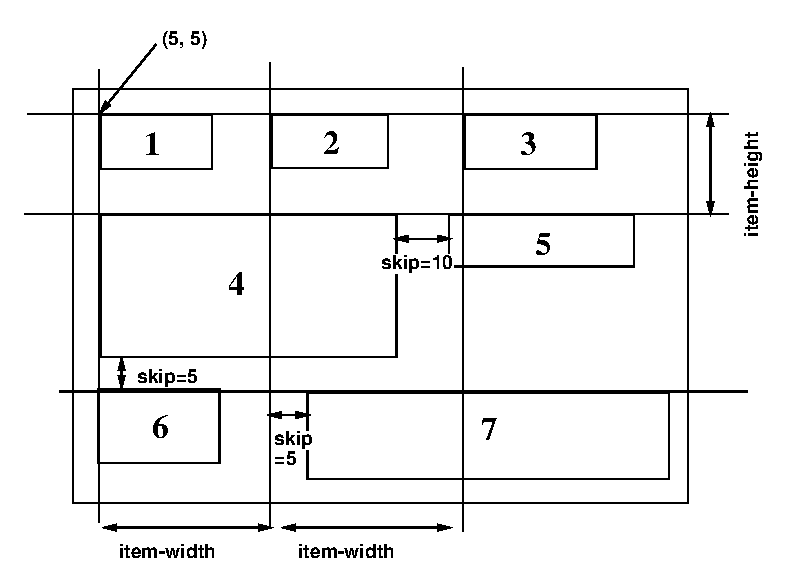
\includegraphics[height=7cm]{fig/panellayout.ps}
%\epsfile{file=fig/panellayout.ps,height=7cm}
\end{center}
\caption{panelのアイテムレイアウト\label{panellayout}}
\end{figure}

\longdescription{:create-item}{klass label receiver method \= \&rest args
\` [メソッド]\\
\> \&key ((:font fontid)\\
\> \&allow-other-keys)}{
{\em klass}で指定されるパネルアイテムのクラス
(すなわち、{\tt button-item,  menu-button-item, slider-item, joystick-item}など),
のインスタンスを作り、{\tt :locate-item}を用いてpanelにアイテムを置く。
{\em args}は、{\em klass}の{\tt :create}メソッドに送られる。
{\em label}は、パネルアイテムの中に書かれる識別文字列である。
{\em receiver}と{\em method}は、一致するイベントを呼び出すイベントハンドラを
指定する。}

\methoddesc{:delete-items}{}{パネルアイテムを全て削除する。}
\longdescription{:create-menubar}{ \= \&rest args \`[メソッド]\\
\> \&key (:font fontid)\\
\> \&allow-other-keys}{
{\em menubar-panel}を作成し、panelの最上部に置く。}
\end{refdesc}

以下に示すメソッドは、イベントがイベントハンドラのないpanelに送られたとき、
"subclass's responsibility"警告メッセージを避けるために提供されている。
ユーザーのアプリケーションでは、これらのメソッドを上書きしなければならない。

\begin{refdesc}
\methoddesc{:quit}{\&rest a}{
{\bf window-main-loop}に{\tt :quit}メッセージを送り、
イベント処理を停止する。}
\methoddesc{:KeyPress}{event}{NILを返す。}
\methoddesc{:KeyRelease}{event}{NILを返す。}
\methoddesc{:ButtonPress}{event}{NILを返す。}
\methoddesc{:ButtonRelease}{event}{NILを返す。}
\methoddesc{:MotionNotify}{event}{NILを返す。}
\methoddesc{:EnterNotify}{event}{NILを返す。}
\methoddesc{:LeaveNotify}{event}{NILを返す。}
\end{refdesc}

\subsubsection{サブパネル(メニューとメニューバー)}

\begin{refdesc}
% menu-panel
\classdesc{menu-panel}{panel}{
 (items item-dots item-height\\
                \>charwidth charheight\\
                \>height-offset\\
                \>highlight-item\\
                \>color-pixels\\
                \>active-color)
}{
{\bf menu-panel}は、{\tt panel-button}と{\tt menu-item}のみを
含むことができるパネルの一種である。
{\tt panel}と異なり、{\tt menu-panel}はふつう見えないし、
{\tt menu-panel}と関連した{\tt button-item}が押された時に
表示される。
もし、menu-panelがいつも見えるように作られたならば、
ピンを刺したメニューとなる。
マウスイベントに対するmenu-itemの応答は、アイテムの外のどこかで
押されたマウスボタンのようにふつうのmenu-buttonと
全く異なっている。
{\tt menu-panel}を使用するためには、最初に作成し、
その中にbutton-itemを置く。
それから、{\tt menu-button-item}がpanelの中あるいはmenubarの中に
{\em :menu}の引数として{\tt menu-panel}と一緒に作成される。}

\longdescription{:create}{\&rest args \= \&key\= (:items) (:border-width 0)
   (:font font-courb12)
\` [メソッド]\\
\>\> (:width 100) (:height-offset 15) (:color *bisque1*)
                      (:active *bisque2*) \\
           \>\&allow-other-keys) 
  }{
{\bf menu-panel} windowを作成する。
そのwindowの大きさは、新しいmenu-itemが追加される時に
拡張される。}

\methoddesc{:add-item}{label name \&optional (receiver self)  \&rest mesg}{
この{\bf menu-panel} windowの中にmenuアイテムを追加し、
対応する行動を張り付ける。
マウスボタンがアイテムの上で外されたとき、
{\em receiver}オブジェクトは{\em mesg}を受け取る。}

% \methoddesc{:popup}{x y \&optional (offset 20)}{
% pops up the menu at the position (x,y) specified on the root window.}
% \methoddesc{:buttonPress}{event}{
% maps the menu-panel  and makes it visible.}
%\methoddesc{:buttonRelease}{event}{
%perform a method coresdonding toa selected item and unmap the menu window.
%}

\classdesc{menubar-panel}{panel}{}{
{\tt menubar-panel}は、親panelの最上部にいつも置かれるサブパネルである。
メニューバーに置かれるパネルアイテムは、{\tt menu-button-item}で
なければならない。
menubar-panelは、panelの{\tt :create-menubar}メソッドにより
生成される。}

\end{refdesc}

\subsubsection{ファイルパネル}
FilePanelは、ファイルやディレクトリを対話的に処理する
アプリケーションwindowである。
{\tt cd}や{\tt go-up}ボタンを使用することにより、
どんなディレクトリも見に行くことができるし、
以下の{\tt ScrollTextWindow}の中にディレクトリ内に含まれるファイルを
表示する。
テキストファイルは、異なったwindow(TextViewPanel)の中に
表示することができる。
ファイルは、また印刷することができ、削除することができ、
ボタンをクリックすることにより簡単にコンパイルすることができる。
ファイルを印刷するとき、{\tt a2ps {\em file} | lpr}コマンドがforkされたプロセスとして実行される。

\begin{figure}
\begin{center}
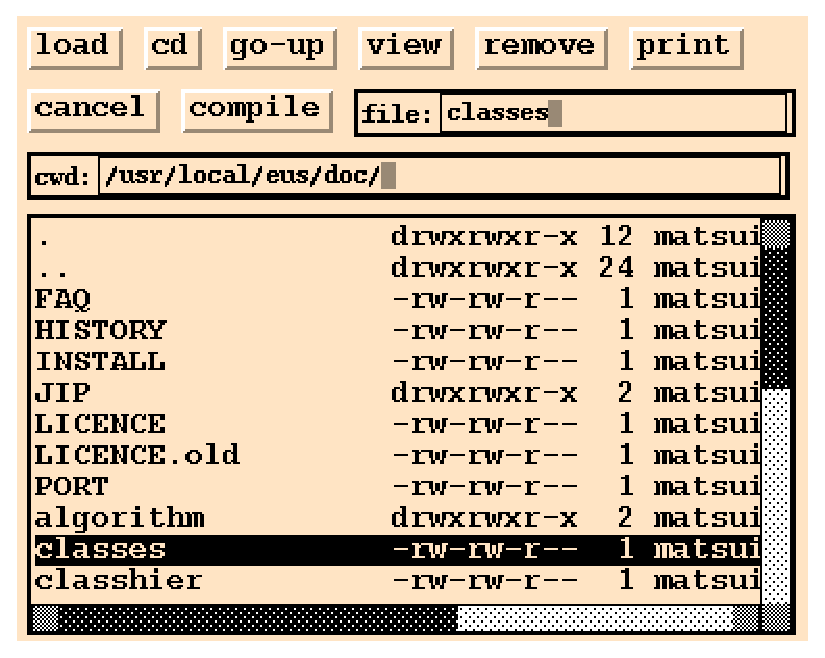
\includegraphics[height=7.5cm]{fig/filepanel.ps}
%\epsfile{file=fig/filepanel.ps,height=7.5cm}
\end{center}
\caption{ファイルパネルwindow}
\end{figure}

\subsubsection{テキスト表示パネル}

TextViewPanelは、テキストファイルを表示するための
アプリケーションwindowクラスである
(図 \ref{textviewpanel})。
プログラムテキストは、もっとも簡単なアプリケーションwindowの1つが
どのように記述されているかを見れる。
{\tt :create}メソッドにおいて、quitボタンとfindボタンと
ファイルの中を捜すための文字列を供給するためのtext-itemを
作成する。
view-windowは、縦と横にスクロールバーを持ちファイルを表示するための
ScrollTextWindowである。
TextViewPanelは、windowマネージャーにより一番外側のタイトルwindowの
大きさを変えたときview-windowの大きさを変えるために
{\tt :ConfigureNotify}イベントを捕獲する。

\begin{figure}
\begin{center}
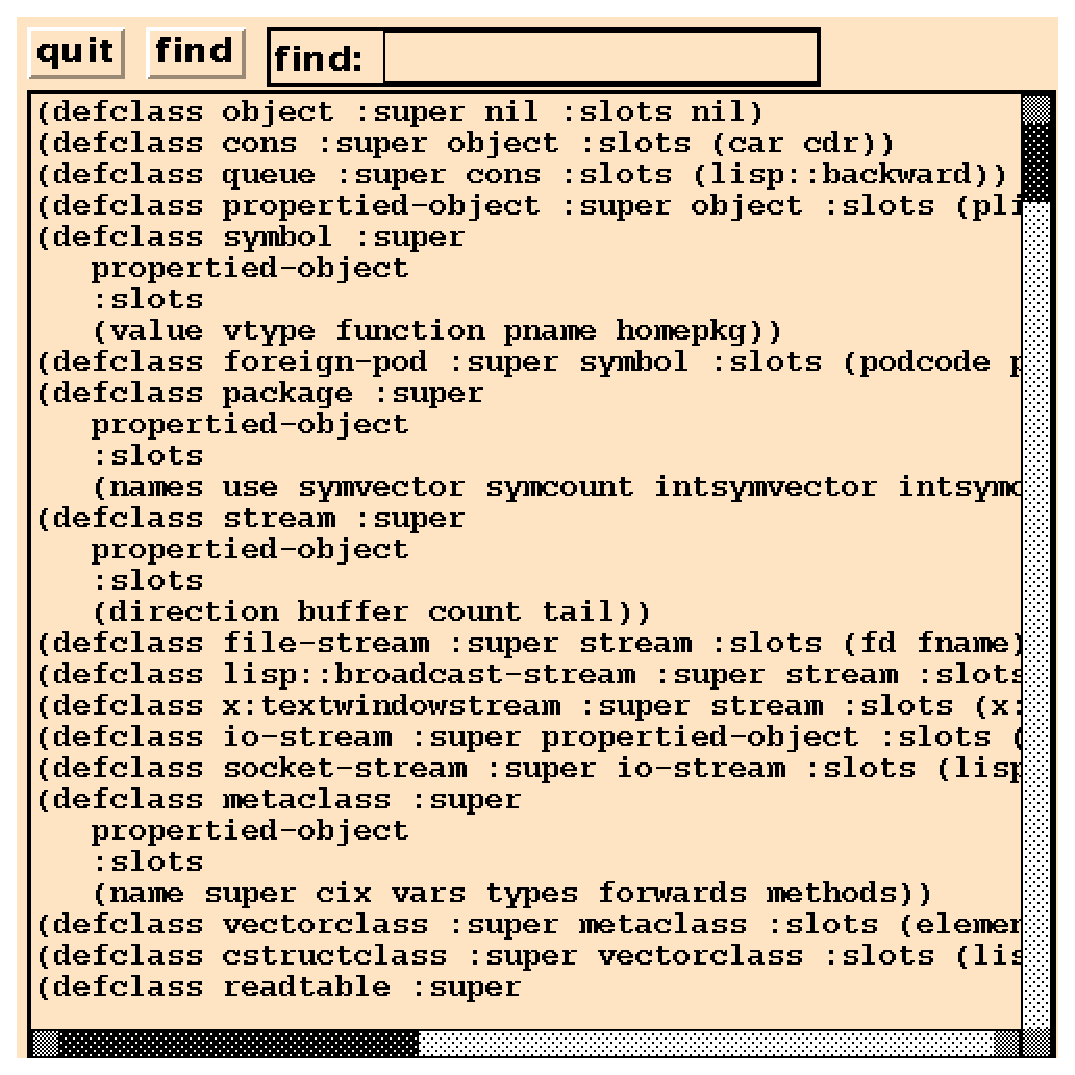
\includegraphics[height=7cm]{fig/textviewpanel.ps}
%\epsfile{file=fig/textviewpanel.ps,height=7cm}
\end{center}
\caption{テキスト表示パネルwindow\label{textviewpanel}}
\end{figure}

\begin{verbatim}
(defclass TextViewPanel :super panel
        :slots (quit-button find-button find-text view-window))

(defmethod TextViewPanel
 (:create (file &rest args &key (width 400) &allow-other-keys)
    (send-super* :create :width width args)
    (setq quit-button
          (send self :create-item panel-button "quit" self :quit))
    (setq find-button
          (send self :create-item panel-button "find" self :find))
    (setq find-text
          (send self :create-item text-item "find: " self :find))
    (setq view-window
            (send self :locate-item
                (instance ScrollTextWindow :create
                   :width (setq width (- (send self :width) 10))
                   :height (- (setq height (send self :height)) 38)
                   :scroll-bar t :horizontal-scroll-bar t
                   :map nil      :parent self)))
    (send view-window :read-file file))
 (:quit (event)  (send self :destroy))
 (:find (event)
    (let ((findstr (send find-text :value)) (found)
          (nlines (send view-window :nlines)))
        (do ((i 0 (1+ i)))
            ((or (>= i nlines) found))
           (if (substringp findstr (send view-window :line i)) (setq found i)))
        (when found
           (send view-window :display-selection found)
           (send view-window :locate found))))
 (:resize (w h)
    (setq width w height h)
    (send view-window :resize (- w 10) (- h 38)))
 (:configureNotify (event)
   (let ((newwidth (send self :width))
         (newheight (send self :height)))
        (when (or (/= newwidth width) (/= newheight height))
          (send self :resize newwidth newheight)))  ) )
\end{verbatim}

\subsection{パネルアイテム}
\begin{refdesc}
\classdesc{panel-item}{xwindow}
{(pos notify-object notify-method\\
\>fontid label labeldots)}{
{\bf panel-item}は、パネルアイテムwindowのすべての種類において、
アイテムが指定するイベントが発生したとき
{\tt notify-object}の{\tt notify-method}を呼び出すための
抽象クラスである。
}

\methoddesc{:notify}{\&rest args}{
{\tt notify-object}の{\tt notify-method}を呼び出す。
イベント応答や{\tt notify-method}へ送るための引き数が
アイテムにより区別される。
\begin{description}
\item [button-item] ボタンは、同じbutton-itemの押し、外し時に応答。
引き数はbutton-itemオブジェクトである。
\item [menu-button-item] メニューアイテムの選択時に応答。
引き数は、menu-button-itemオブジェクトである。
\item [choice-item] 新しい選択ボタンの選択時に応答。
引き数は、choice-itemオブジェクトとその選択番号である。
\item [text-item] 改行あるいはリターンの入力時に応答。
引き数は、text-itemオブジェクトと入力行(文字列)である。
\item [slider-item] スライダーノブは、つかみと移動時に応答。
引き数は、slider-itemオブジェクトと新たな値である。
\item [joystick-item] ジョイスティックは、つかみと移動時に応答。
引き数はslider-itemオブジェクトと新しいxとyの値である。
\end{description}
}

\longdescription{:create}{name reciever method \= \&rest args
\` [メソッド] \\
\> \&key ((:width w) 100) ((:height h) 100) (:font font-courb12)\\
\> \&allow-other-keys}{
パネルアイテムを作成する。
パネルアイテムは、抽象クラスである。
このメソッドは、サブクラスによって{\tt send-super}を通してのみ
呼び出すべきである。}

\classdesc{button-item}{panel-item}{}{
{\bf button-item}は、簡単なパネルアイテムである。
button-itemは、四角ボックスとその中のラベル文字列を持っている。
クリックされたとき、button-itemはpanel-itemオブジェクトを唯一の引き数として
{\tt notify-object}の{\tt notify-method}
を呼び出す。}

\methoddesc{:draw-label}{\&optional (state :top) (color bg-color) (border 2) (offset)}{
{\bf button-item}のラベルを書く。}

\longdescription{:create}{label revciever method \= \&rest args
\` [メソッド]\\
\>\&key\= :width :height (:font (send parent :gc :font))\\
\>\> (:background (send parent :gc :background)) \\
\>\> (:border-width 0) \\
\>\> (:state :top)\\
\>\&allow-other-keys}{
{\bf button-item}を作成する。
もし、ボタンの幅と高さが与えられないなら、サイズは
与えられたフォントを用いて書かれた
ラベル文字列に合わせて自動的に設定される。
{\em :border-width}はデフォルトで0であるが、
擬似3次元表現でボタンを浮き出しにする。
背景やフォントは親window(すなわち、panel)で定義されているものを
デフォルトとする。}

\methoddesc{:ButtonPress}{event}{
もし、ボタンであれば、背景色をグレーにする。}

\methoddesc{:ButtonRelease}{event}{
{\em event}の背景色を標準に変更する。}


\classdesc{menu-button-item}{button-item}{(\= items item-dots item-labels\\
\>charwidth charheight \\
\>menu-window window-pos high-light)
}{
プルダウンメニューを定義する。
{\bf menu-button-item}は、{\tt button-item}のようであるが、
{\bf menu-button-item}は、ボタンの下の関連する{\tt menu-panel}が
押されたとき、
{\tt notify-object}にすぐにメッセージを送る代わりに、
活性化させる。
メニューアイテムの1つの上でマウスボタンが外されたときに、本当のメッセージが
送られる。}

\longdescription{:create}{\= label reciever method \` [メソッド]\\
\>\&rest args\\
\>\&key (:menu nil) (:items) (:state :flat)\\
\>\&allow-other-keys}{
プルダウンメニューを作成する。
{\em receiver}と{\em method}引き数は、影響を与えない。}

\methoddesc{:ButtonPress}{event}{
プルダウンメニューのボタンを反転させ、
ボタンの下に関連するmenu-panelをさらす。}

\methoddesc{:ButtonRelease}{event}{
このボタンの下の{\tt menu-panel}を消し、
このボタンを元に戻す。}

% Bitmap-button-item
\classdesc{bitmap-button-item}{button-item}{
(pixmap-id bitmap-width bitmap-height)
}{
{\bf bitmap-button-item}の関数は、{\tt button-item}に似ているが、
表現が異なっている。
{\tt button-item}の場合にボタンの上に簡単なラベル文字列を描く代わりに、
{\tt bitmap-button-item}では、ボタンが作られたときにbitmapファイルから
ロードされるpixmapを描く。}

\longdescription{:create}{ bitmap-file reciever method \= \&rest args
\` [メソッド]\\
                 \>\&key :width :height\\
                 \>\&allow-other-keys)
}{
{\bf bitmap-button-item}を作成する。
最初の引き数{\em bitmap-file}は、{\tt button-item}の{\em label}引き数
を置き換えたものである。}

\methoddesc{:draw-label}{\&optional (state :flat) (color bg-color) (border 2)}{
ボタンの上にbitmapかpixmapを描く。}

\methoddesc{:create-bitmap-from-file}{fname}{
{\em fname}という名のbitmapファイルからpixmapを作り、
{\tt pixmap-id}にそのIDを入れる。}

% choice-item
\classdesc{choice-item}{button-item}{
 (choice-list active-choice transient-choice \\
                \>choice-dots choice-pos button-size)
}{
{\bf choice-item}は、丸い選択ボタンの集合である。
1つの選択はいつも活性化しており、同時に1つの選択だけが
活性化することができる。
{\bf choice-item}は、ラジオボタンと同様な機能を提供する。}

\longdescription{:create}{label reciever method \= \&rest args
\` [メソッド]\\
           \>\&key \=(:choices '("0" "1")) (:initial-choice 0)\\
\>\> (:font (send parent :gc :font))\\
                \>\>(:button-size 13)\\
                \>\>(:border-width 0)\\
  }{
{\bf choice-item-button}を作成する。
それぞれの選択ボタンは{\em :button-size}の半径を持つ円である。
新しい選択ボタンが選択されたとき、
{\tt notify-object}の{\tt notify-method}が
choice-itemオブジェクトと選択された選択ボタンの番号と一緒に呼び出される。}

\methoddesc{:value}{\&optional (new-choice) (invocation)}{
もし、{\em new-choice}が与えられたならば、現在の活性化選択ボタンとして
設定し、対応する円が黒色になる。
もし{\em  invocation}も指定されているなら、{\tt notify-object}の
{\tt notify-method}が呼び出される。
{\tt :value}は、現在の(あるいは新しい)選択ボタンの番号を返す。}

\methoddesc{:draw-active-button}{\&optional
(old-choice active-choice) (new-choice active-choice)}{
ボタンを活性化として書く。
}

\methoddesc{:ButtonPress}{event}{
もし、選択ボタンのどこかでマウスボタンが押されているなら、
その番号が{\tt transient-choice}に記録される。
マウスボタンが外されるまでそれ以上の行動は、起こさない。}

\methoddesc{:ButtonRelease}{event}{
もし、既に押されていたところと同じボタンの上でマウスボタンが外されたなら、
{\tt active-choice}が更新され、
{\tt notify-object}の{\tt notify-method}が呼び出される。
}

% Slider-item
\classdesc{slider-item}{panel-item}{
(min-value max-value value\\
                \>minlabel maxlabel valueformat\\
                \>bar-x bar-y bar-width bar-height valuedots label-base\\
                \>nob-x nob-moving\\
                \>charwidth) 
}{
{\tt choice-item}が離散的な値の選択に使用されるのに対し、
{\bf slider-item}は{\tt min-value}と{\tt max-value}の間の範囲の
連続的な値に対して使用される。
それぞれ値が変化した瞬間、slider-itemオブジェクトと新しい値が引き数として
一緒に{\tt notify-object}の{\tt notify-method}が呼び出される。}

\longdescription{:create}{label reciever method \= \&rest args
\` [メソッド]\\
\>\&key (:min 0.0) (:max 1.0) (:parent)\\
\>(:min-label "") (:max-label "") (:value-format "~4,2f")\\
\>(:font font-courb12) (:span 100) (:border-width 0) (:initial-value min)  }{
{\bf slider-item}を作成する。
スライドのノブは、バーの上に小さな黒の四角として表示される。
左端が{\em :min}値を表現し、右端が{\em :max}値を表現する。
バーの長さは、{\em :span}ドットに引き伸ばす。
現在の値は、{\em :value-format}でslider-itemの右に表示する。}

\methoddesc{:value}{\&optional newval invocation}{
もし、{\em newval}が与えられたなら、現在の値として設定され、
ノブは対応する位置にスライドする。
もし、{\em invocation}もnon NILに指定されていたなら、
{\tt notify-object}の{\tt notify-method}が呼び出される。
{\tt :value}は、現在の(新しい)値を返す。}

% JoyStick-item
\classdesc{joystick-item}{panel-item}{
 (stick-size min-x min-y max-x max-y\\
                \>center-x center-y stick-x stick-y\\
                \>value-x value-y\\
                \>stick-return stick-grabbed\\
                \>fraction-x fraction-y)
}{
{\bf joystick-item}は、2次元のslider-itemとしてみなすことができる。
2つの連続値はクモの巣のような同心円図の上を動く黒い円によって
指定することができる(図 \ref{panelitem})。}

\longdescription{:create}{name reciever method \= \&rest args
\` [メソッド]\\
           \>\&key \=(:stick-size 5) (:return nil)\\
                \>\>(:min-x -1.0) (:max-x 1.0)\\
                \>\>(:min-y -1.0) (:max-y 1.0)\\
           \>\&allow-other-keys) 
  }{
{\em :stick-size}は、スティックの黒い円の半径である。
同心円図の円の大きさは、{\bf joystick-item} windowの幅と高さ
に合うように決定される。
もし、{\em :return}がnon NILであるなら、
ジョイスティックは、マウスボタンが外された時の原点に帰る。
そうでないなら、ジョイスティックは、外された位置に残る。}


%\methoddesc{:draw-circles}{}{
%}
%\methoddesc{:xy}{\&optional (x value-x) (y value-y)}{
%}
%\methoddesc{:draw-stick}{\&optional (x value-x) (y value-y) (erase t)}{
%}
\methoddesc{:value}{\&optional (newx) (newy) (invocation)}{
もし、{\em newx}と{\em newy}が与えられたなら、
現在の位置として設定され、ジョイスティックは同心円図の
対応する位置に移動する。
もし、{\em invocation}もnon NILに指定されたなら、
{\tt notify-object}の{\tt notify-method}が、
{\bf joystick-item}オブジェクトとx,y値を引き数として一緒に呼び出される。
{\tt :value}は、現在の(新しい)値のリストを返す。}

\end{refdesc}

以下に上に記述されているpanel-itemを使った短いプログラムを示し、
図 \ref{panelitem}がパネルの中にどのように表示されるかを示したものである。

\begin{verbatim}
(in-package "X")
(defclass testPanel :super panel
        :slots (quit joy choi sli))
(defmethod testPanel
 (:create (&rest args)
    (send-super* :create :width 210 :height 180 
                 :font font-courb12 args)
    (send-super :create-item button-item "quit" self :quit :font font-courb14)
    (send-super :create-item choice-item "choice" self :choice
                :choices '(" A " " B " " C ")
                :font font-courb12)
    (send-super :create-item slider-item "slider" self :slider
                :span 90)
    (send-super :create-item joystick-item "joy" self :joy)
    self)
 (:choice (obj c) (format t "choice: ~S ~d~%" obj c))
 (:slider (obj val) (format t "slider: ~S ~s~%" obj val))
 (:joy (obj x y) (format t "joy: ~S ~s ~s~%" obj x y)) )
(instance testPanel :create)
(window-main-thread)
\end{verbatim}

\begin{figure}
\begin{center}
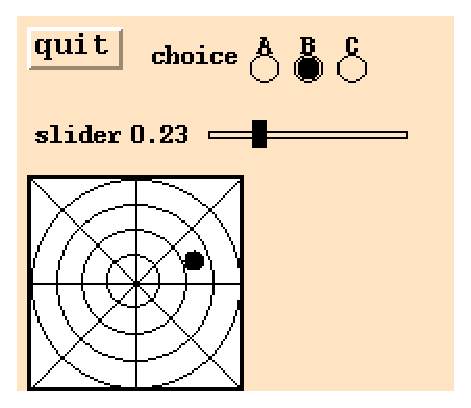
\includegraphics[height=5cm]{fig/panelitem.ps}
%\epsfile{file=fig/panelitem.ps,height=5cm}
\end{center}
\caption{panelの中に作成されたpanel-item\label{panelitem}}
\end{figure}

\begin{refdesc}
\classdesc{text-item}{panel-item}
{(textwin)}{
{\bf text-item}は、ファイル名のような短いテキストを表示したり入力したり
するために使用する。
{\bf text-item}は、ラベル文字列とその右側に小さなテキストwindowを持っている。
テキストwindow内にポインタが置かれたとき、キー入力が可能となり、
入力された文字がバッファに入れられる。
テキストwindow内の行修正が可能である。
{\tt control-F}と{\tt control-B}は前後に1文字動かし、
{\tt del}はカーソルの左の1文字を削除し、
{\tt control-D}はカーソル位置の文字を削除し、
カーソル位置にはどんなグラフィック文字も挿入できる。
マウスボタンをクリックすれば、クリックされた文字にカーソルを
移動させる。
enter(改行)キーを打つことにより、バッファされたテキストが
{\tt notify-object}の{\tt notify-method}に送られる。}

\longdescription{:create}{label revciever method \= \&rest args \` [メソッド]\\
\>\&key (:font font-courb12) (:columns 20) (:initial-value ) (:border-width 0)\\
\>\&allow-other-keys}{
{\bf text-item}を作成する。
テキストwindowの行バッファには、長さの制限が無いけれども、
見える部分は{\em columns}文字に制限されている。}

\methoddesc{:getstring}{}{
キーバッファ内の文字列を返す。}

%\methoddesc{:KeyPress}{pos}{
%if key is pressed, print key character to cursor position.}

%\methoddesc{:keyEnter}{ch}{
%prints {\em ch} to cursor position. But if {\em ch} is backspace,
%deletes 1 character from buffer. And if {\em ch} is return or newline,
%ignores.}
\end{refdesc}

\subsection{キャンバス}
\begin{refdesc}
\classdesc{canvas}{xwindow}{(topleft bottomright)}{
{\bf canvas}は、図や画像を入れるためのXwindowである。
現在、領域選択機能のみ実現されている。
ButtonPressイベントにより、{\bf canvas}は押された位置を左上の端とし、
現在の位置を右下の端とする四角を描き始める。
ButtonReleaseにより、{\tt notify-object}の{\tt notify-method}が
送られる。
canvas内に図や画像を描くためにはXdrawableのメソッドが使用される。}

%\methoddesc{:adjust-corners}{}{
%corrects toleft and bottomright.}

%\methoddesc{:region-selection}{}{
%prints canvas region.}

%\methoddesc{:draw-selection-rectangle}{}{
%draws a rectangle that shows canvas region.}

%\methoddesc{:ButtonPress}{event}{
%reverses the color of button that shows {\em event}.}
%\methoddesc{:MotionNotify}{event}{
%makes selection rectangle which corners are pressed position 
%and cursor position.}
%\methoddesc{:ButtonRelease}{event}{
%clears selection rectangle and prints item on this canvas region.}

%\methoddesc{:clear-canvas}{item}{
%ignores {\em item}.}

\end{refdesc}

\subsection{テキストwindow}

{\tt TextWindow}と{\tt BufferTextWidnow}と{\tt ScrollTextWindow}の
3つのテキストwindowがある。

\begin{refdesc}
\classdesc{textWindow}{xwindow}
{(fontid \\
\>charwidth charheight charascent dots \\
\>win-row-max win-col-max \\
\>win-row win-col \hspace{20mm} \= ;physical current position in window \\
\>x y\\
\>charbuf \>; for charcode conversion \\
\>keybuf keycount \> ;for key input\\
\>echo \\
\>show-cursor cursor-on \> ;boolean\\
\>kill delete \> ;control character \\
\>notify-object notify-method \\
\>)}{
メッセージを表示するために使用可能な仮想端末を実現する。
表示される内容は、バッファされないし、{\bf TextWindow}に既に表示された
文字や行を引き出す方法はない。
基本的に、{\bf TextWindow}は
カーソル移動、行削除、領域削除、表示テキストのスクロール、文字列挿入
などを持つダンプ端末と似た能力を持っている。
また、テキストカーソルはマウスポインタで指示された位置に
移動することができる。}

\methoddesc{:init}{id}{
{\em id}番目のテキストwindowを初期化する。}

\longdescription{:create}{\=\&rest args \` [メソッド]\\
\>\&key \=:width :height (:font font-courb14) :rows :columns\\
\>(:show-cursor nil) (:notify-object nil) (:notify-method nil)\\
\>\&allow-other-keys}{
text-windowを作成する。
windowの大きさは、{\em :width}と{\em :height}かあるいは{\em :rows}と
{\em :columns}で指定されたものとなる。
{\em :notify-object}の{\em :notify-method}は、改行文字が入力された
ときに呼び出される。}

%\methoddesc{:set-notify}{reciever method}{
%}

\methoddesc{:cursor}{flag}{
{\em flag}は、{\tt :on, :off, :toggle}のどれかが可能である。
テキストカーソルは、{\tt win-row}と{\tt win-col}の位置である。
もし、{\em flag}が{\tt :on}であれば、テキストカーソルは表示され、
{\em flag}が{\tt :off}ならば、消される。
また、{\em flag}が{\tt toggle}ならば、反対になる。
このメソッドは、カーソルの位置の文字を更新するときはいつでも、
呼び出されなければならない。}

\methoddesc{:clear}{}{
テキストwindow内を消去する。}

\methoddesc{:clear-eol}{\&optional (r win-row) (c win-col) (csr :on)}{
{\em r}と{\em c}で指定される位置の文字以降の残りの行を
消去する。カーソル位置の文字も含む。}

\methoddesc{:clear-lines}{lines \&optional (r win-row)}{
{\em r}番目の行以降の複数行を消去する。}

\methoddesc{:clear-eos}{\&optional (r win-row) (c win-col)}{
{\em r}と{\em c}で指定される位置から画面の最後までの領域を消去する。}

\methoddesc{:win-row-max}{}{このwindowに表示可能な最大行数を返す。}

\methoddesc{:win-col-max}{}{このwindowに表示可能な最大列数を返す。}

\methoddesc{:xy}{\&optional (r win-row) (c win-col)}{
{\em r}と{\em c}で指定される位置の文字のピクセル座標を計算する。}

\methoddesc{:goto}{r c \&optional (cursor :on)}{
{\em r}番目の行の{\em c}番目の列にカーソルを移動する。}

\methoddesc{:goback}{\&optional (csr :on)}{
カーソルを1文字戻す。}

\methoddesc{:advance}{\&optional (n 1)}{
{\em n}文字だけカーソルを進める。}

\methoddesc{:scroll}{\&optional (n 1)}{
{\em n}行だけ縦方向にテキストwindowをスクロールする。}

\methoddesc{:horizontal-scroll}{\&optional (n 1)}{
{\em n}列だけ横方向にテキストをスクロールする。}

\methoddesc{:newline}{}{
次の行の最初にカーソルを移動する。}

\methoddesc{:putch}{ch}{
カーソル位置に文字{\em ch}を挿入する。
行の残りは、1文字前方に進められる。}

%\methoddesc{:putstr}{str \&optional (e (length str))}{
%prints {\em str} to text-window.}
%
\methoddesc{:putstring}{str \&optional (e (length str))}{
カーソル位置に{\em str}を置く。}

%\methoddesc{:getstring}{}{gets key-buffer.}

\methoddesc{:event-row}{event}{}
\methoddesc{:event-col}{event}{
{\em event}における、テキストカーソルの位置をを返す。}
%\methoddesc{:EnterNotify}{event}{}
%\methoddesc{:ButtonPress}{event}{}
%\methoddesc{:ButtonRelease}{event}{}
%\methoddesc{:resize}{w h}{}
%\methoddesc{:ConfigureNotify}{event}{}
%\methoddesc{:keyrelease}{}{nob}
%\methoddesc{:enterNotify}{event}{}
%\methoddesc{:LeaveNotify}{event}{}
\methoddesc{:KeyPress}{event}{
カーソル位置に入力された文字を挿入する。
もし、文字が改行であったなら、{\tt notify-object}に通知する。}
%\methoddesc{:keyEnter}{ch}{}
%\methoddesc{:LineEnter}{ch}{}
%\methoddesc{:clear-text}{item}{clear text-window.}

\classdesc{TextWindowStream}{stream}{(textwin)}{
{\tt TextWindowStream}は、TextWdinowに接続された出力ストリームである。
{\tt print, format, write-byte}などによってこのストリームに出力
される文字や文字列がTextWdindowに表示される。
通常のファイルストリームとしては、
出力データはバッファされる。}

\methoddesc{:flush}{}{
バッファされたテキスト文字列を掃き出し、TextWindowに送る。
{\tt finish-output}やこのストリームへの改行文字の書き込みは、
このメソッドを自動的に呼び出す。}

\funcdesc{make-text-window-stream}{xwin}{
{\bf text-window-stream}を作り、そのストリームオブジェクトを返す。}

\classdesc{BufferTextWindow}{TextWindow}{
(linebuf expbuf max-line-length row col)}{
{\bf TextWindow}の内容を表現する行バッファを保持する。
{\tt linebuf}は、行のベクトルである。{\tt exbuf}は、
タブ拡張されたテキストを持つ。
windowに表示可能な行のみが保持される。
{\bf BufferTextWindow}は、数行のテキストを持つ
簡単なテキストエディタとして使用することができる。
{\tt text-item}は、表示可能な行バッファとして{\bf BufferTextWindow}を
使う。}

%\methoddesc{:create}{\&rest args}{}
%\methoddesc{:clear}{}{}
%\methoddesc{:goto}{r c \&optional (csr :on)}{}
\methoddesc{:line}{n}{
{\em n}番目の行の内容を文字列として返す。}

\methoddesc{:nlines}{}{{\tt linebuf}の行数を返す。}
\methoddesc{:all-lines}{}{文字列のベクトルである{\tt linebuf}を返す。}
\methoddesc{:refresh-line}{\&optional (r win-row) (c win-col)}{
{\em r}番目の行の{\em c}番目の列以降を再書き込みする。}
\methoddesc{:refresh}{\&optional (start 0)}{
{\em start}番目の行以降の行を再書き込みする。}
\methoddesc{:insert-string}{string}{
カーソル位置に{\em string}を挿入する。}
\methoddesc{:insert}{ch}{カーソル位置に文字を挿入する。}
\methoddesc{:delete}{n}{カーソル以降の{\em n}文字を削除する。}
%\methoddesc{:KeyEnter}{ch \&optional event}{}
%\methoddesc{:ButtonRelease}{event}{}

\funcdesc{expand-tab}{src \&optional (offset 0)}{
{\em src}は、タブを含んだ可能性のある文字列である。
これらのタブは、タブの停止位置が8の倍数であると仮定して空白文字に
置き換えられる。}

\classdesc{ScrollTextWindow}{BufferTextWindow}{
(top-row top-col \hspace{30mm} \= ;display-starting position \\
\> scroll-bar-window \\
\> horizontal-scroll-bar-window \\
\> selected-line)}{
{\bf ScrollTextWindow}は、行数制限がなく、縦と横にスクロールバーを持った
{\tt BufferTextWindow}を定義する。
{\bf ScrollTextWindow}は、スクロールバーを伴ってwindowの大きさを変更するため、
あるいはテキストを再表示するために{\tt :configureNotify}イベントを
扱うことができる。
クリックすることによって、行を選択することができる。}

\methoddesc{:create}{\&rest args
           \&key (scroll-bar nil)
                (horizontal-scroll-bar nil)
           \&allow-other-keys}{
スクロールバーが必要なとき、それぞれのキーワードの引き数にTを指定する。}

%\methoddesc{:locate-scroll-bar}{}{}
%\methoddesc{:clear}{}{}
%\methoddesc{:lines}{}{}
%\methoddesc{:max-line-length}{}{}
%\methoddesc{:refresh}{\&optional (offset 0) (lines (- win-row-max offset))}{}
%\methoddesc{:line-in-window-p}{ln}{}
%\methoddesc{:refresh-line}{ln \&optional (highlight nil) \&aux fg-save bg-save}{
%}
\methoddesc{:locate}{n}{windowの上部から{\em n}番目の行に
バッファされたテキストを表示する。}
\methoddesc{:display-selection}{selection}{
{\em selection}は、選択された行の位置を表現する。
選択された行がすべて高輝度で表示される。}

\methoddesc{:selection}{}{選択された行(文字列)を返す。}

\methoddesc{:read-file}{fname}{
{\em fname}で指定されるテキストファイルを{\tt linebuf}に読み込み、
タブを拡張し、windowに表示する。
カーソルは、画面の最初に置かれる。}

\methoddesc{:display-string}{strings}{
{\em strings}は、行(文字列)の列である。
{\em strings}は、{\tt linebuf}にコピーされ、windowに表示される。}

%\methoddesc{:scroll-fraction}{}{}
%\methoddesc{:horizontal-scroll-fraction}{}{}

\methoddesc{:scroll}{n}{{\em n}行、縦にスクロールする。}
\methoddesc{:horizontal-scroll}{n}{{\em n}列、横にスクロールする。}
%\methoddesc{:insert-char}{c \&optional (refresh t)}{}
%\methoddesc{:insert-newline}{\&optional (refresh t)}{}
%\methoddesc{:insert}{thing \&optional (refresh t)}{}
%\methoddesc{:buttonPress}{event}{}
\methoddesc{:ButtonRelease}{event}{
マウスポインタが置かれている行が選択される。
もし、windowが作成されたときに{\tt notification}が指定されている
ならば、{\tt notify-object}の{\tt notify-method}が呼び出される。}

\methoddesc{:resize}{w h}{
windowの大きさを変更し、新しいサイズに合うように
内容を再表示する。
もし、スクロールバーがあれば、同じメッセージが送られる。}
%\methoddesc{:ConfigureNotify}{event}{}

%\classdesc{xitem}{xwindow}
%{(label labeldots width height)}{
%defines xitem that is used for pulldown menu.}

%\methoddesc{:draw-label}{}{
%draws xitem's label.}

%\longdescription{:create}{label \= \&rest args \hspace{120mm} [method]\\
%\>\&key width height (font font-cour10)\\
%\>\&allow-other-keys}{
%creates xitem.}

% \classdesc{input-panel}{panel}{}{
% defines input-lines for panel. Input-panel is a one line input window that
% has quit button, cancel button and input line with under-line. 
% This class is used by xinput function.}
% 
% \methoddesc{:getstring}{}{
% gets key-buffer.}
% 
% \methoddesc{:quit}{\&rest args}{
% quit this input line window.}
% 
% \methoddesc{:input-line}{\&rest args}{
% quit this input line window.}
% 
% \methoddesc{:create}{title len \&rest args}{
% creates input line window. And add 'CANCEL' button on this window.}
% 
%\funcdesc{xitem-length}{label \&key (font font-cour10)}{
%returns {\em label}'s length.}

%\funcdesc{xset-eachground}{win fg bg \&optional (f-flag t)}{
%sets {\em win}'s foreground color and background color. And {\em win} refresh.
%But if {\em f-flag} is nil, {\em win} don't refresh.}

% \funcdesc{x::xinput}{\&key (title "Input:") (len 30) (font font-cour10) (par *root*) x y}{
% creates input-panel positioned ({\em x},{\em y}), then gets string. 
% If input is end, returns input string, and destroys this input-panel. 
% When input string is nothing, returns nil. Notes that mouse cursor have
% to be moved on the input area, whenever you input text.}

\end{refdesc}

\newpage
